\documentclass[../lecture-notes-148x210.tex]{subfiles}

\begin{document}

\subsection{R1CS in Matrix Form}

While the Rank-1 Constraint System provides a powerful way to represent computations, it is not 
succinct at all, since the number of constraints depends linearly on the complexity of the problem 
being solved. In practical scenarios, this can require tens or even hundreds of thousands of 
constraints, sometimes even millions. The Quadratic Arithmetic Program (QAP) can address this issue.

\begin{remark}
    Understanding polynomials and their properties is crucial for this section.
    If you are not confident in this area, it is better to revisit the
    corresponding chapter and refresh your knowledge. See
    \Cref{section:polynomial-rings}.
\end{remark}

To define a constraint in the R1CS we need four vectors: three coefficient
vectors ($\boldsymbol{\ell}$, $\boldsymbol{r}$, and $\boldsymbol{o}$) and the
witness one --- $\mathbf{z}$. And that's just for one constraint. As you can
imagine, many of the values in these vectors are zeros. In circuits with
thousands of inputs, outputs, and auxiliary variables, where there are also
thousands of constraints, you could end up with a millions of zeroes.

\begin{remark}
    A matrix in which most of the elements are zero in numerical analysis is
    usually called \textbf{sparse matrix}.
\end{remark}

So, we need to change the way how we manage coefficients and make the
representation of such matrices and vectors succint (as required by the
definition of SNARK).

\begin{theorem}[R1CS in the Matrix Form]
    Consider a Rank-1 Constraint System (R1CS) defined by $m$ constraints. Each
    constraint is associated with coefficient vectors $\boldsymbol{\ell}_i$,
    $\boldsymbol{r}_i$, and $\boldsymbol{o}_i$, where $i \in [m]$. Suppose a
    witness vector $\mathbf{z}$ consists of $n$ elements. Then, this system can
    also be represented using the corresponding $m \times n$ matrices $L,R,O$
    such that all constraints can be reduced to the single equation:
    \begin{equation*}
        L\mathbf{z} \odot R\mathbf{z} = O\mathbf{z}
    \end{equation*}
    
    In this representation:
    \begin{itemize}
        \item Each $i$-th row of the matrices corresponds to the coefficients of a specific constraint.
        \item Each column of these matrices corresponds to the coefficients
        associated with a particular element of the witness vector $\mathbf{z}$.
    \end{itemize}
\end{theorem}

\textbf{Proof.} Matrices defined this way can be expressed as
\begin{equation*}
    L = \begin{bmatrix}
        \boldsymbol{\ell}_1^{\top} \\ \boldsymbol{\ell}_2^{\top} \\ \vdots \\ \boldsymbol{\ell}_m^{\top}
    \end{bmatrix}, \quad R = \begin{bmatrix}
        \boldsymbol{r}_1^{\top} \\ \boldsymbol{r}_2^{\top} \\ \vdots \\ \boldsymbol{r}_m^{\top}
    \end{bmatrix}, \quad O = \begin{bmatrix}
        \boldsymbol{o}_1^{\top} \\ \boldsymbol{o}_2^{\top} \\ \vdots \\ \boldsymbol{o}_m^{\top}
    \end{bmatrix}
\end{equation*}

Consider an expression $L\mathbf{z}$:
\begin{equation*}
    L\mathbf{z} = \begin{bmatrix}
        \boldsymbol{\ell}_1^{\top} \\ \boldsymbol{\ell}_2^{\top} \\ \vdots \\ \boldsymbol{\ell}_m^{\top}
    \end{bmatrix}\begin{bmatrix}
        z_1 \\ z_2 \\ \vdots \\ z_n
    \end{bmatrix} = \begin{bmatrix}
        \boldsymbol{\ell}_1^{\top}\mathbf{z} \\ \boldsymbol{\ell}_2^{\top}\mathbf{z} \\ \vdots \\ \boldsymbol{\ell}_m^{\top}\mathbf{z}
    \end{bmatrix}
\end{equation*}

The last equality is a bit tricky to observe, so let us explain how we ended up with such expression. Notice that since $L \in \mathbb{F}^{m \times n}$ and $\mathbf{z} \in \mathbb{F}^n$, the product $L\mathbf{z}$ is a vector from $\mathbb{F}^m$. Now, for $j^{\text{th}}$ element of such vector, based on the matrix product definition, we have $(L\mathbf{z})_j = \sum_{\ell=1}^na_{j,\ell}z_{\ell}$ which is exactly an inner product between $\boldsymbol{\ell}_j$ and $\mathbf{z}$! Therefore, we have:
\begin{equation*}
    L\mathbf{z} = \begin{bmatrix}
        \langle \boldsymbol{\ell}_1, \mathbf{z}\rangle \\
        \langle \boldsymbol{\ell}_2, \mathbf{z}\rangle \\
        \vdots \\
        \langle \boldsymbol{\ell}_m, \mathbf{z}\rangle 
    \end{bmatrix}, \quad
    R\mathbf{z} = \begin{bmatrix}
        \langle \boldsymbol{r}_1, \mathbf{z}\rangle \\
        \langle \boldsymbol{r}_2, \mathbf{z}\rangle \\
        \vdots \\
        \langle \boldsymbol{r}_m, \mathbf{z}\rangle 
    \end{bmatrix}, \quad
    O\mathbf{z} = \begin{bmatrix}
        \langle \boldsymbol{o}_1, \mathbf{z}\rangle \\
        \langle \boldsymbol{o}_2, \mathbf{z}\rangle \\
        \vdots \\
        \langle \boldsymbol{o}_m, \mathbf{z}\rangle 
    \end{bmatrix}
\end{equation*}

Therefore, $L\mathbf{z} \odot R\mathbf{z} = O\mathbf{z}$ is equivalent to the system of $m$ constraints:
\begin{equation*}
    \langle \boldsymbol{\ell}_j, \mathbf{z}\rangle \times \langle \boldsymbol{r}_j, \mathbf{z} \rangle = \langle \boldsymbol{o}_j, \mathbf{z} \rangle, \; j \in [m].
\end{equation*}

\begin{example}
    The vectors $\boldsymbol{\ell}_i$ from the previous examples have the form:
    \begin{align*}
        \boldsymbol{\ell}_1 &= (0, 0, 1, 0, 0, 0, 0) \\
        \boldsymbol{\ell}_2 &= (0, 0, 0, 1, 0, 0, 0) \\
        \boldsymbol{\ell}_3 &= (0, 0, 1, 0, 0, 0, 0) \\
        \boldsymbol{\ell}_4 &= (1, 0, -1, 0, 0, 0, 0)
    \end{align*}
    This corresponds to $n = 7, m = 4$
    \begin{equation*}
        \scalebox{0.9}{$
        L = \begin{bmatrix}
            L_{1,1} & L_{1,2} & L_{1,3} & L_{1,4} & L_{1,5} & L_{1,6} & L_{1,7} \\
            L_{2,1} & L_{2,2} & L_{2,3} & L_{2,4} & L_{2,5} & L_{2,6} & L_{2,7} \\
            L_{3,1} & L_{3,2} & L_{3,3} & L_{3,4} & L_{3,5} & L_{3,6} & L_{3,7} \\
            L_{4,1} & L_{4,2} & L_{4,3} & L_{4,4} & L_{4,5} & L_{4,6} & L_{4,7}
        \end{bmatrix} = \begin{bmatrix}
            0 & 0 & 1 & 0 & 0 & 0 & 0 \\
            0 & 0 & 0 & 1 & 0 & 0 & 0 \\
            0 & 0 & 1 & 0 & 0 & 0 & 0 \\
            1 & 0 & -1 & 0 & 0 & 0 & 0 
        \end{bmatrix}
        $}
    \end{equation*}
\end{example}

\subsection{Polynomial Interpolation}

Now is the time to define how we are going to build polynomials! Notice that the
columns of these matrices (say, column $(\ell_{1,i},\ell_{2,i},\ell_{3,i},\ell_{4,i})$ in
matrix $L$ from example above) represent the mappings from constraint number $i$
to the corresponding coefficient of the $j$ element in the witness vector!

\begin{example}
    Consider the witness from the previous examples: 
    \begin{equation*}
        \mathbf{z} = (1, r, x_1, x_2, x_3, \mathsf{mult}, \mathsf{selectMult})
    \end{equation*}
    For element $x_1$ we are interested in the third columns of the $L$, $R$ and $O$ matrices, as
    it's placed on the third position in the witness vector, so $j = 3$.\\
    For matrix $L$:
    \begin{center}
        \begin{tikzpicture}
            % Node to contain the pmatrix
            \node (L) at (0,0) {$
                \begin{bmatrix}
                    0 & 0 & \textcolor{red!100}{1} & 0 & 0 & 0 & 0 \\
                    0 & 0 & \textcolor{red!100}{0} & 1 & 0 & 0 & 0 \\
                    0 & 0 & \textcolor{red!100}{1} & 0 & 0 & 0 & 0 \\
                    1 & 0 & \textcolor{red!100}{-1} & 0 & 0 & 0 & 0 \\
                \end{bmatrix}
            $};
        
        \end{tikzpicture}
    \end{center}

    Thus, for constraint number 4 ($i = 4$) the coefficient of $x_1$ is $-1$:
    \begin{center}
        \begin{tikzpicture}
            % Node to contain the pmatrix
            \node (L) at (0,0) {$
                \begin{bmatrix}
                    0 & 0 & \textcolor{red!100}{1} & 0 & 0 & 0 & 0 \\
                    0 & 0 & \textcolor{red!100}{0} & 1 & 0 & 0 & 0 \\
                    0 & 0 & \textcolor{red!100}{1} & 0 & 0 & 0 & 0 \\
                    \textcolor{blue!100}{1} & \textcolor{blue!100}{0} & \textcolor{black!100}{-1} & \textcolor{blue!100}{0} & \textcolor{blue!100}{0} & \textcolor{blue!100}{0} & \textcolor{blue!100}{0} \\
                \end{bmatrix}
            $};
        
        \end{tikzpicture}
    \end{center}
\end{example}
Good, so now we know that for the $j$th element in the witness vector there are $m$ (the number of constraints) corresponding values in matrices $L$, $R$, and $O$. Now, we want to encode this statement in a form of a polynomial. 
As we know from the previous chapters, such a mapping in math can be built using the Lagrange polynomial interpolation.

\begin{remark}
    As a remainder, the Lagrange interpolation polynomial $f(X) \in
    \mathbb{F}^{\leq n}[X]$ for a given set of points
    $\{(x_0,y_0),(x_1,y_1),\dots,(x_n,y_n)\} \subseteq \mathbb{F} \times
    \mathbb{F}$ such that $f(x_i)=y_i$ can be built with the following formula:
    \begin{equation*}
        f(X) = \sum_{i=0}^{n} y_i e_i(X), \quad e_i(X) = \prod_{j=0, j \neq i}^{n} \frac{X-x_j}{x_i-x_j}.
    \end{equation*}  
\end{remark}

For a given column $j \in [n]$ in a matrix $L$ the set of points that define the
variable polynomial $\ell_j(X)$ can be defined as $\{(i, L_{i,j})\}_{i \in
[m]}$. In other words, we want to interpolate $n$ polynomials $\ell_j(X) \in
\mathbb{F}[X]$ such that:
\begin{equation*}
    \ell_j(i) = L_{i,j}, \; i \in [m], \; j \in [n].
\end{equation*}

The same is true for matrices $R$ and $O$, resulting in $3n$ polynomials, $n$ for each of the
coefficients matrices:
\begin{align*}
    \ell_1(X), \ell_2(X), \dots, \ell_n(x), 
    r_1(X), r_2(X), \dots, r_n(X),
    o_1(X), o_2(X), \dots, o_n(X)
\end{align*}

\begin{example}
    Considering the witness vector $\mathbf{z}$ and matrix $L$ from the previous example, for the variable
    $x_1$, the next set of points can be derived:
    \begin{equation*}
        \{(1,1), (2,0), (3,1), (4,-1)\}
    \end{equation*}
    We can see that it is used in the 1st, 3rd, and 4th constraints as the values of the coefficients
    are not zero.
    
    The Lagrange interpolation polynomial for this set of points can be built as
    follows (for the demonstration purposes, assume we are working over
    $\mathbb{R}$):
    \begin{align*}
        e_1(X) &= \frac{(X - 2)(X - 3)(X - 4)}{(1 - 2)(1 - 3)(1 - 4)} = -\frac{(X - 2)(X - 3)(X - 4)}{6}, \\
        e_2(X) &= \frac{(X - 1)(X - 3)(X - 4)}{(2 - 1)(2 - 3)(2 - 4)} = \frac{(X - 1)(X - 3)(X - 4)}{2}, \\
        e_3(X) &= \frac{(X - 1)(X - 2)(X - 4)}{(3 - 1)(3 - 2)(3 - 4)} = -\frac{(X - 1)(X - 2)(X - 4)}{2}, \\
        e_4(X) &= \frac{(X - 1)(X - 2)(X - 3)}{(4 - 1)(4 - 2)(4 - 3)} = \frac{(X - 1)(X - 2)(X - 3)}{6}.
    \end{align*}

    Thus, the polynomial is given by:
    \begin{equation*}
        \begin{aligned}
            \ell_1(X) &= 1 \cdot e_1(X) + 0 \cdot e_2(X) + 1 \cdot e_3(X) + (-1) \cdot e_4(X) \\
            &= -\frac{(X - 2)(X - 3)(X - 4)}{6} - \frac{(X - 1)(X - 2)(X - 4)}{2} - \\ 
            &- \frac{(X - 1)(X - 2)(X - 3)}{6} = -\frac{5}{6}X^3 + 6X^2 - \frac{79}{6}X + 9.
        \end{aligned}
    \end{equation*}
    Therefore, the final Lagrange interpolation polynomial is:
    \begin{equation*}
        \ell_1(X) = -\frac{5}{6}X^3 + 6X^2 - \frac{79}{6}X + 9
    \end{equation*}

    As shown in Illustration below, the curve intersects all the given points.
    In this figure, the $x$-axis represents the constraint number, and the
    $y$-axis represents the coefficients of the $x_1$ witness element.

    \begin{center}
        \scalebox{0.8}{
        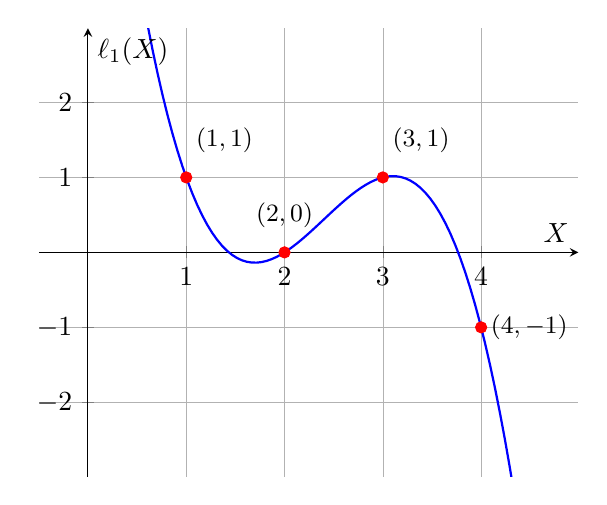
\begin{tikzpicture}
            \begin{axis}[
                axis lines = middle,
                xlabel = {$X$},
                ylabel = {$\ell_1(X)$},
                ymin = -2.99, ymax = 2.99,
                xmin = -0.5, xmax = 4.99,
                domain = 0:5,
                samples = 100,
                ytick = {-3,...,3},
                xtick = {0,1,...,5},
                grid = both, 
                grid style = {line width=.1pt, draw=gray!20},
                major grid style = {line width=.2pt, draw=gray!60}
            ]
            \addplot[
                color=blue,
                thick
            ]
            {-5/6*x^3 + 6*x^2 - 79/6*x + 9};
            \addplot[
                only marks,
                mark=*,
                color=red
            ]
            coordinates {(1,1) (2,0) (3,1) (4,-1)};
    
            \node at (axis cs:1,1.5) [anchor=west] {\small $(1,1)$};
            \node at (axis cs:2,0.2) [anchor=south] {\small $(2,0)$};
            \node at (axis cs:3,1.5) [anchor=west] {\small $(3,1)$};
            \node at (axis cs:4,-1) [anchor=west] {\small $(4,-1)$};
            
            \end{axis}
        \end{tikzpicture}
        }

        \textbf{Illustration:} The Lagrange inteprolation polynomial for points $\{(1,1), (2,0), (3,1), (4,-1)\}$ visualized over $\mathbb{R}$.
    \end{center}
\end{example}

\begin{remark}
    One might a reasonable question: why do we choose $x$-coordinates to be the
    indeces of the corresponding constraints? Actually, just for convenience
    purposes. We could have assigned any \textit{unique} index from $\mathbb{F}$
    to each constraint (say, $t_i$ for each $i \in [m]$) and interpolate through
    these points:
    \begin{equation*}
        \ell_j(t_i) = L_{i,j}, \; i \in [m], \; j \in [n]
    \end{equation*}

    As we will see in the subsequent lectures, we can define the $x$-coordinates
    in much more clever way to reduce the workload needed for interpolation. But
    for now, we will stick to this simple version.
\end{remark}


\subsection{Putting All Together!}

Now, using coefficients encoded with polynomials, a constraint number $h \in
[m]$, from a constraint system with a witness vector $\mathbf{z}$ can be built
in the next way:
\begin{equation*} 
    \scalebox{0.9}{$
    \begin{aligned}
        (z_1\ell_1(h) + z_2\ell_2(h) + \dots + z_n\ell_n(h)) &\times (z_1r_1(h) + z_2r_2(h) + \dots + z_nr_n(h)) =\\ = (z_1o_1(h) + z_2o_2(h)& + \dots + z_no_n(h))
    \end{aligned}
    $}
\end{equation*}

Or, written more concisely:
\begin{equation*}
    \sum_{i \in [n]} z_i\ell_i(h) \cdot \sum_{i \in [n]} z_ir_i(h) = \sum_{i \in [n]} z_io_i(h).
\end{equation*}

\begin{remark}
    Hold on, but why does it hold? Let us substitute any $X=j$ into this equation:
    \begin{equation*}
        \sum_{i \in [n]} z_i\ell_i(j) \cdot \sum_{i \in [n]} z_ir_i(j) = \sum_{i \in [n]} z_io_i(j) \; \forall j \in [m]
    \end{equation*}

    Recall that we interpolated polynomials to have $\ell_i(j) = L_{j,i}$.
    Therefore, the equation above can be reduced to:
    \begin{equation*}
        \sum_{i \in [n]} z_iL_{j,i} \cdot \sum_{i \in [n]} z_iR_{j,i} = \sum_{i \in [n]} z_iO_{j,i} \; \forall j \in [m]
    \end{equation*}

    But hold on again! Notice that $\sum_{i \in [n]} z_iL_{j,i} = \langle \mathbf{z}, \boldsymbol{\ell}_j \rangle$ and therefore we have:
    \begin{equation*}
        \langle \mathbf{z}, \boldsymbol{\ell}_j \rangle \times \langle \mathbf{z}, \boldsymbol{r}_j \rangle = \langle \mathbf{z}, \boldsymbol{o}_j \rangle \; \forall j \in [m],
    \end{equation*}
    so we ended up with the initial $m$ constraint equations!
\end{remark}

Now let us define polynomials $\ell(X)$, $r(X)$, $o(X)$ for easier notation: 
\begin{equation*}
    \ell(X) = \sum_{i \in [n]} z_i\ell_i(X), \quad r(X) = \sum_{i \in [n]} z_ir_i(X), \quad o(X) = \sum_{i \in [n]} z_io_i(X)
\end{equation*}

Therefore, our set of constraints can be rewritten simply as the single check
$\ell(h)\cdot r(h) = o(h)$ for each $h \in [m]$ --- much less scary-looking than
what we have written before. OK, but what does it give us? 

Notice that if $\ell(X) \cdot r(X)=o(X)$ for all $h \in [m]$ then polynomial,
defined as $m(X) := \ell(X) \cdot r(X) - o(X)$, has zeros at all elements from
the set $\Omega = [m]$. Define the so-called \textbf{vanishing polynomial} on
$\Omega$ as:
\begin{equation*}
    z_{\Omega}(X) := \prod_{h \in \Omega} (X - h) = \prod_{i \in [m]} (X - i)
\end{equation*} 

Now, if $m(X)$ vanishes on all points from $\Omega$, it means that $z_{\Omega}$
must divide $m$, so $z_{\Omega} \mid m$. But that means that $m$ can be divided
by $z_{\Omega}$ without remainder! In other words, there exists some polynomial
$h$ such that $m=z_{\Omega}h$. We further drop index $\Omega$ for simplicity. 

All in all, let us give the definition of a \textbf{Quadratic Arithmetic Program}.

\begin{definition}[Quadratic Arithmetic Program]
    Suppose that $m$ R1CS constraints with a witness of size $n$ are written in a form
    \begin{equation*}
        L\mathbf{z} \odot R\mathbf{z} = O\mathbf{z}, \; L,R,O \in \mathbb{F}^{m \times n}
    \end{equation*}

    Then, the \textbf{Quadratic Arithmetic Program} consists of $3n$ polynomials
    $\ell_1,\dots,\ell_n$, $r_1,\dots,r_n$, $o_1,\dots,o_n$ such that:
    \begin{equation*}
        \ell_j(i) = a_{i,j}, \; r_j(i) = b_{i,j}, \; o_j(i) = c_{i,j}, \; \forall i \in [m] \; \forall j \in [n]
    \end{equation*}

    Then, $\mathbf{z} \in \mathbb{F}^n$ is a valid assignment for the given QAP
    and \textbf{target polynomial} $z(X) = \prod_{i \in [m]} (X-i)$ if and only
    if there exists such a polynomial $h(X)$ such that
    \begin{equation*}
        \sum_{i \in [n]} z_i\ell_i(X) \cdot \sum_{i \in [n]} z_ir_i(X) - \sum_{i \in [n]} z_io_i(X) = z(X)h(X)
    \end{equation*}
\end{definition}

This was our final step in representing a high-level programming language to some math primitive.
We have managed to encode our computation to a single polynomial!

\subsection{Probabilistically Checkable Proofs}

Before going further we should get acquainted with one more concept from the computational 
complexity theory, that have an important application in zk-SNARK and provides the theoretical 
backbone. 

L Probabilistically Checkable Proof (PCP) is a type of proof system where the verifier can 
efficiently check the correctness of a proof by examining only a small, random portion of it, rather
than verifying it entirely. 
\begin{definition}
    L language $\mathcal{L} \subseteq \Sigma^*$ (for some given alphabet
    $\Sigma$) is in the class $\mathsf{PCP}(r,q)$ (\textbf{probabilistically
    checkable proofs}), where $r$ is the \emph{randomness complexity} and $q$ is
    the \emph{query complexity}, if for a given pair of algorithms
    $(\mathcal{P}, \mathcal{V})$: 
    \begin{itemize}
        \item \emph{Syntax:} $\mathcal{P}$ calculates a proof (bit string) $\pi
        \in \Sigma^*$ in polynomial time $\mathsf{poly}(|\mathbbm{x}|)$ of the
        common input $\mathbbm{x}$. The prover $\mathcal{P}$ and verifier
        $\mathcal{V}$ interact, where the verifier has an oracle access to $\pi$
        (meaning, he queries it at any position).
        \item \emph{Complexity:} $\mathcal{V}$ uses at most $r$ random bits to
        decide which part of the proof to query and the verifier queries at most
        $q$ bits of the proof.
    \end{itemize}
    
    Such pair of algorithms $(\mathcal{P}, \mathcal{V})$ should satisfy the
    following properties (with a security parameter $\lambda \in \mathbb{N}$):
    \begin{itemize}
        \item \textbf{Completeness}: If $\mathbbm{x} \in \mathcal{L}$, then $\Pr[\mathcal{V}^{\pi}(\mathbbm{x}) = 1] = 1$.
        \item \textbf{Soundness}: If $\mathbbm{x} \notin \mathcal{L}$, then for
        any possible (malicious) proof $\pi^*$, 
        \begin{equation*}
            \Pr[\mathcal{V}^{\pi^*}(\mathbbm{x}) = 1] = \mathsf{negl}(\lambda).
        \end{equation*}
    \end{itemize}
\end{definition}
This allows a verification of huge statements with high confidence while using
limited computational resources. See \Cref{fig:pcp}.

\begin{theorem}{\textbf{PCP theorem (PCP characterization theorem)}\\} Any
    decision problem in $\mathsf{NP}$ has a PCP verifier that uses logarithmic
    randomness $O(\log n)$ and a constant number of queries $O(1)$, independent
    of $n$.
    \begin{equation*}
        \mathsf{NP} = \mathsf{PCP}(O(\log n), O(1))
    \end{equation*}
\end{theorem}

\begin{figure}[h!]
    \centering

    \scalebox{0.8}{
    \begin{tikzpicture}
        \node[inner sep=0pt, align=center] at (-4.0, 0.0) (prover) {
\includegraphics[width=1.25cm]{lectures/images/common/prover.png}\\Prover $\mathcal{P}$};
        \node[inner sep=0pt, align=center] at (4.0, 0.0) (verifier) {
\includegraphics[width=1.25cm]{lectures/images/common/verifier.png}\\Verifier $\mathcal{V}$};

        \draw[fill=gray!20!white, ultra thick] (-2.0, 4) rectangle (2.0, 3.25);

        % Query boxes
        \draw[fill=blue!60!white, ultra thick] (-1.0, 4) rectangle (-0.8, 3.25);
        \node at (-0.9, 4.35) (pcp) {$q_1$};
        \draw[fill=blue!60!white, ultra thick] (0.0, 4) rectangle (0.2, 3.25);
        \node at (0.1, 4.35) (pcp) {$q_2$};
        \draw[fill=blue!60!white, ultra thick] (0.5, 4) rectangle (0.7, 3.25);
        \node at (0.6, 4.35) (pcp) {$q_3$};
        \node at (0, 2.85) (pcp) {\textbf{PCP Oracle}};

        \draw[-{Stealth[length=3mm]},line width=0.4mm] (prover)--(pcp) node[midway, left=3mm]{Generate an oracle ($\pi$)};
        \draw[-{Stealth[length=3mm]},line width=0.4mm] (verifier)--(pcp) node[midway, right=3mm]{Point queries $q_1,\dots,q_m$};
    \end{tikzpicture}
    }

    \caption{Illustration of a Probabilistically Checkable Proof (PCP) system. The prover $\mathcal{P}$ generates a PCP oracle $\pi$ that is queried by the verifier $\mathcal{V}$ at specific points $q_1,\dots,q_m$.}
    \label{fig:pcp}
\end{figure}

However, despite the fact that PCP is a very powerful tool, it is not used
directly in zk-SNARKs. We need to extend it a bit to make it more suitable for
our purposes.

Three main extensions of PCPs that are frequently used in SNARKs are:
\begin{itemize}
    \item \textbf{IPCP} (\textbf{Interactive PCP}): The prover commits to the PCP oracle and then, based on the interaction between the prover and verifier, the verifier queries the oracle and decides whether to accept the proof.
    \item \textbf{IOP} (\textbf{Interactive Oracle Proof}): The prover and verifier interact and on each round, the prover commits to a new oracle. The verifier queries the oracle and decides whether to accept the proof.
    \item \textbf{LPCP} (\textbf{Linear PCP}): The prover commits to a linear function and the verifier queries the function at specific points.
\end{itemize}

\begin{figure}[h!]
    \centering

    \scalebox{0.75}{
    \begin{tikzpicture}
        \node[inner sep=0pt, align=center] at (-4.0, 0.0) (prover) {
\includegraphics[width=1.25cm]{lectures/images/common/prover.png}\\Prover $\mathcal{P}$};
        \node[inner sep=0pt, align=center] at (4.0, 0.0) (verifier) {
\includegraphics[width=1.25cm]{lectures/images/common/verifier.png}\\Verifier $\mathcal{V}$};

        % Oracle 1
        \node at (-2.0, 5.625) (oracle_1_left) {};
        \node at (2.0, 5.625) (oracle_1_right) {};
        \draw[fill=gray!20!white, ultra thick] (-2.0, 6) rectangle (2.0, 5.25);
        \draw[fill=blue!60!white, ultra thick] (-1.0, 6) rectangle (-0.8, 5.25);
        \node at (-0.9, 6.35) (pcp) {$q_1$};
        \draw[fill=blue!60!white, ultra thick] (0.0, 6) rectangle (0.2, 5.25);
        \node at (0.1, 6.35) (pcp) {$q_2$};
        \draw[fill=blue!60!white, ultra thick] (0.5, 6) rectangle (0.7, 5.25);
        \node at (0.6, 6.35) (pcp) {$q_3$};
        \node at (0, 4.85) (pcp) {\textbf{PCP Oracle \#1}};

        % Oracle 2
        \node at (-2.0, 3.625) (oracle_2_left) {};
        \node at (2.0, 3.625) (oracle_2_right) {};
        \draw[fill=gray!20!white, ultra thick] (-2.0, 4) rectangle (2.0, 3.25);
        \draw[fill=blue!60!white, ultra thick] (-0.4, 4) rectangle (-0.2, 3.25);
        \node at (-0.3, 4.35) (pcp) {$q_1'$};
        \draw[fill=blue!60!white, ultra thick] (0.2, 4) rectangle (0.4, 3.25);
        \node at (0.3, 4.35) (pcp) {$q_2'$};
        \draw[fill=blue!60!white, ultra thick] (1.5, 4) rectangle (1.7, 3.25);
        \node at (1.6, 4.35) (pcp) {$q_3'$};
        \node at (0, 2.85) (pcp) {\textbf{PCP Oracle \#2}};

        % Oracle 3
        \node at (-2.0, 1.625) (oracle_3_left) {};
        \node at (2.0, 1.625) (oracle_3_right) {};
        \draw[fill=gray!20!white, ultra thick] (-2.0, 2) rectangle (2.0, 1.25);
        \draw[fill=blue!60!white, ultra thick] (-1.5, 2) rectangle (-1.3, 1.25);
        \node at (-1.4, 2.35) (pcp) {$q_1''$};
        \draw[fill=blue!60!white, ultra thick] (0.3, 2) rectangle (0.5, 1.25);
        \node at (0.4, 2.35) (pcp) {$q_2''$};
        \draw[fill=blue!60!white, ultra thick] (1.0, 2) rectangle (1.2, 1.25);
        \node at (1.1, 2.35) (pcp) {$q_3''$};
        \node at (0, 0.85) (pcp) {\textbf{PCP Oracle \#3}};

        \draw[-{Stealth[length=3mm]},line width=0.4mm] (prover)--(oracle_1_left) node[midway, left=3mm]{Commit to oracles ($\pi_1,\dots,\pi_r$)};
        \draw[-{Stealth[length=3mm]},line width=0.4mm] (verifier)--(oracle_1_right) node[midway, right=3mm]{Point queries ($\mathbf{q}_1,\dots,\mathbf{q}_r$)};
        \draw[-{Stealth[length=3mm]},line width=0.4mm] (prover)--(oracle_2_left) node[midway, left=3mm]{};
        \draw[-{Stealth[length=3mm]},line width=0.4mm] (verifier)--(oracle_2_right) node[midway, right=3mm]{};
        \draw[-{Stealth[length=3mm]},line width=0.4mm] (prover)--(oracle_3_left) node[midway, left=3mm]{};        
        \draw[-{Stealth[length=3mm]},line width=0.4mm] (verifier)--(oracle_3_right) node[midway, right=3mm]{};

        % Two arrows to left and to right between the prover and verifier with the "Interaction" label
        \draw[{Stealth[length=3mm]}-{Stealth[length=3mm]},line width=0.4mm,dashed] (prover) to node[midway, below]{Interaction} (verifier);
    \end{tikzpicture}
    }
    \caption{Illustration of an Interactive Oracle Proof (IOP). On each round $i$ ($1 \leq i \leq r$), $\mathcal{V}$ sends a message $m_i$, and $\mathcal{P}$ commits to a new oracle $\pi_i$, which $\mathcal{V}$ can query at $\mathbf{q}_i=(q_{i,1},\dots,q_{i,m})$.}
    \label{fig:pcp}
\end{figure}

While IOPs will be later used for PLONK and zk-STARKs, we will focus on Linear
PCPs in the context of Groth16 zk-SNARK. Let us define it below.

\begin{definition}[Linear PCP]
    L \textbf{Linear PCP} is a PCP where the prover commits to a linear function
    $\boldsymbol{\pi} = (\pi_1,\dots,\pi_k)$ and the verifier queries the
    function at specific points $\boldsymbol{q}_1,\dots,\boldsymbol{q}_r$. Then,
    the prover responds with the values of the function at these points:
    \begin{equation*}
        \langle \boldsymbol{\pi}_1, \mathbf{q}_1 \rangle, \langle \boldsymbol{\pi}_2, \mathbf{q}_2 \rangle, \dots, \langle \boldsymbol{\pi}_r, \mathbf{q}_r \rangle.
    \end{equation*}
\end{definition}

\begin{example}[QAP as a Linear PCP]
    Recall that key QAP equation is:
    \begin{equation*}
        \sum_{i \in [n]}z_i\ell_i(X) \cdot \sum_{i \in [n]}z_ir_i(X) - \sum_{i \in [n]}z_io_i(X) = z(X)h(X).
    \end{equation*}

    Now, the notation might be confusing, but firstly, we denote vectors of polynomials: 
    \begin{align*}
        \boldsymbol{\ell}(X) & = (\ell_1(X),\dots,\ell_n(X)), \\
        \boldsymbol{r}(X) & = (r_1(X),\dots,r_n(X)), \\
        \boldsymbol{o}(X) & = (o_1(X),\dots,o_n(X)).
    \end{align*}
    
    Now, consider the following \textbf{linear PCP for QAP}:
    \begin{enumerate}
        \item $\mathcal{P}$ commits to an extended witness $\mathbf{z}$ and
        coefficients $\mathbf{h} = (h_1,\dots,h_n)$ of $h(X)$.
        \item $\mathcal{V}$ samples $\gamma \leftarrowS \mathbb{F}$ and sends
        query $\boldsymbol{\gamma} = (\gamma,\gamma^2,\dots,\gamma^n)$ to
        $\mathcal{P}$.
        \item $\mathcal{P}$ reveals the following values:
        \begin{equation*}
            \begin{aligned}
                &\pi_1 \gets \langle \mathbf{z}, \boldsymbol{\ell}(\gamma) \rangle, \quad \pi_2 \gets \langle \mathbf{z}, \boldsymbol{r}(\gamma) \rangle, \\
                &\pi_3 \gets \langle \mathbf{z}, \boldsymbol{o}(\gamma) \rangle, \quad \pi_4 \gets z(\gamma) \cdot \langle \mathbf{h}, \boldsymbol{\gamma} \rangle.                
            \end{aligned}
        \end{equation*}
        \item $\mathcal{V}$ checks whether $\pi_1\pi_2 - \pi_3 = \pi_4$.
    \end{enumerate}
\end{example}

Of course, the above example cannot be used as it is: at the very least, we have not specified how the prover commits to the extended witness $\mathbf{z}$ and coefficients $\mathbf{h}$ and then ensures consistency of $\pi_1,\dots,\pi_4$ with these commitments. For that reason, we need some more tools to make it work which we learned in the previous lectures.

\subsection{QAP as a Linear PCP}

When constructing a Quadratic Arithmetic Program (QAP) for a circuit $\Circ$, we
represented the whole circuit's computation using the following relation:
$
% \begin{equation*}
    \ell(X)r(X) - o(X) = z(X)h(X),
% \end{equation*}
$
where by $\ell(X)$, $r(X)$, $o(X)$ we denote the polynomials that represent the
left, right and output wires of the circuit, respectively. $z(X)$ is the target
polynomial, while $h(X) := m(X)\big/z(X)$ for master polynomial $m(X) =
\ell(X)r(X) - o(X)$ is the quotient polynomial.

We effectively managed to transform all the circuit's constraints, and
computations in the short form. It still allows one to verify that each
computational step is preserved by verifying the polynomial evaluation in
specific (random) points, instead of recomputing everything. However, it is not
quite clear why such a check is safe and how it can be used in a PCP. In other
words, why checking that $\ell(s)r(s)-o(s)=z(s)h(s)$ for randomly selected $s$
is enough to verify the circuit $\Circ$?

\textbf{Informal Soundness Justification.} Why is it safe to use such a check?
As it was said early, we perform all the computations in some finite field
$\mathbb{F}$. The polynomials $\ell(X)$, $r(X)$ and $o(X)$ are interpolated
polynomials using $\left| \Circ \right|$ (number of gates) points, so
$\deg(\ell), \deg(r), \deg(o) \leq \left|\Circ\right|$. Thus, using properties
of polynomials' degrees, we can estimate the degree of polynomial $m(X) =
\ell(X)r(X) - o(X)$: $\deg(m) \leq \max\{\deg(\ell) + \deg(r), \deg(o)\} \leq 2
\left| \Circ \right|$. For that reason, when checking the equality
$\ell(s)r(s)-o(s)=z(s)h(s)$ for randomly selected $s$, we can be sure that the
left-hand side and right-hand side polynomials are the same with probability at
least $1-2\left|\Circ\right|/|\mathbb{F}|$.

\end{document}